\documentclass[]{plaid-homework}

% Personal Information
\newcommand{\name}{Sayan Chaudhry, Deepayan Patra}
\newcommand{\andrewid}{\texttt{sayanc, dpatra}}

% Course Settings
\newcommand{\course}{07-131}
\newcommand{\recitation}{A}
\newcommand{\professor}{Cortina}

% Assignment Settings
\newcommand{\homework}{3}

\begin{document} 
\passport{}
\title

\problem{1}{Math}
LaTeX is awesome for math! Let's look evaluating the value of $m$ if $(m + 2) \times (3 + 4) = 21$ in two ways.

Using the initial equality:
\begin{align*}
          && (m + 2) \times (3 + 4) &= 21 \tag{start}
\\\implies&& (m + 2) \times 7 &= 21 \tag{evaluating $3 + 4 = 7$}
\\\implies&& m + 2 &= \frac{21}{7} \tag{dividing by $7$ on both sides}
\\\implies&& m + 2 &= 3 \tag{evaluating $\frac{21}{7} = 3$}
\\\implies&& m &= 3 - 2 \tag{subtracting $2$ on both sides}
\\\implies&& m &= 1 \tag{evaluating $3 - 2 = 1$}
\end{align*}

Therefore:
\[m = 1\]

\starpart

Using the initial equality:
\begin{align*}
          && (m + 2) \times (3 + 4) &= 21 \tag{start}
\\\implies&& (m + 2) \times 7 &= 21 \tag{evaluating $3 + 4 = 7$}
\\\implies&& (m \times 7) + (2 \times 7) &= 21 \tag{using distributive property}
\\\implies&& (m \times 7) + 14 &= 21 \tag{evaluating $2 \times 7 = 14$}
\\\implies&& m \times 7 &= 21 - 14 \tag{subtracting $14$ on both sides}
\\\implies&& m \times 7 &= 7 \tag{evaluating $21 - 14 = 7$}
\\\implies&& m &= \frac{7}{7} \tag{dividing by $7$ on both sides}
\\\implies&& m &= 1 \tag{evaluating $\frac{7}{7} = 1$}
\end{align*}

Therefore:
\[m = 1\]

\newpage

\problem{2}{Induction}
Induction becomes so much easier with LaTeX! Take a look:

\newpage

\problem{2}{Calculus}
Those of you who enjoy calculus will have a blast!

Find $\lim_{x\rightarrow2}\frac{x^2 + x - 6}{x^2 - 4}$.

\begin{align*}
  \lim_{x\rightarrow2}\frac{x^2 + x - 6}{x^2 - 4} &= \lim_{x\rightarrow2}\frac{2x+1}{2x} \tag{by L'Hôpital's Rule}\\
  &= \frac{5}{4}
\end{align*}

Another one? Ok!

Given $f(x,y) = \frac{xy}{x+y}$ if $(x,y) \neq (0,0)$ and $f(0,0) = 0$. 

For $(x,y) \neq (0,0)$, 
\begin{align*}
    \frac{\partial f}{\partial x}(x,y) &= \frac{\partial }{\partial x}\left(\frac{xy}{x+y}\right) \tag{by substitution}\\
    &= \frac{y(x+y)-xy(1)}{(x+y)^2} \tag{by differentiation rules}\\
    &= \frac{y^2}{(x+y)^2}
\end{align*}
and
\begin{align*}
  \frac{\partial f}{\partial y}(x,y) &= \frac{\partial }{\partial y}\left(\frac{xy}{x+y}\right) \tag{by substitution}\\
  &= \frac{x(x+y)-xy(1)}{(x+y)^2} \tag{by differentiation rules}\\
  &= \frac{x^2}{(x+y)^2}
\end{align*}

Alright, no more problems. Just two more equations.
\begin{align*}
  \iiint_{V} (\nabla \cdot \mathbf{F}) \di V
  &= \oiint_{S(V)} \mathbf{F} \cdot \hat{\mathbf{n}} \di S\\
  \iiint_{V} (\nabla \times \mathbf{F}) \di V
  &= \oiint \hat{\mathbf{n}} \times \mathbf{F} \di S
\end{align*}

\newpage

\problem{3}{Programming}

You can code in LaTeX too! Here's an intro to typesetting programs:
\begin{lstlisting}
  #include<stdio.h> 
  #include<iostream>

  // My first program
  int main(void)
  {
    printf("Hello World\n");
    return 0;
  }
\end{lstlisting}
You can also change languages really easily, like here:
\begin{lstlisting}[language=sml]
  (* My second program *)
  fun map f xs = let
    fun m ([], acc) = List.rev acc
      | m (x::xs, acc) = m (xs, f x::acc)
    in
      m (xs, [])
    end
\end{lstlisting}
or here:
\begin{lstlisting}[language=Python]
  # My third program
  def UncommonWords(A, B): 
    # count will contain all the word counts 
    count = {} 
      
    # insert words of string A to hash 
    for word in A.split(): 
      count[word] = count.get(word, 0) + 1
      
    # insert words of string B to hash 
    for word in B.split(): 
      count[word] = count.get(word, 0) + 1
  
    # return required list of words 
    return [word for word in count if count[word] == 1] 
\end{lstlisting}

\newpage

\problem{4}{Graphing}
Plotting in Latex is super fun! Here's a mini graph with some shading:
\begin{center}
  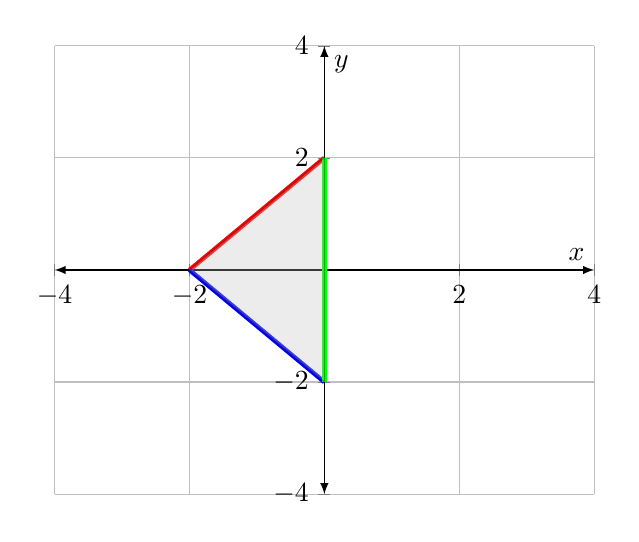
\begin{tikzpicture}
      \begin{axis}[
          grid=both,
          axis x line=center,
          axis y line=center,
          xmin=-4, xmax=4,
          ymin=-4, ymax=4,
          xlabel = $x$,
          ylabel = $y$,
          axis line style={latex-latex}]
          \addplot [domain=-2:0,samples=250, ultra thick, red] {x+2};
          \addplot [domain=-2:0,samples=250, ultra thick, blue] {-x-2};
          \addplot [samples=250, ultra thick, green] coordinates {(0, -2) (0, 2)};
          \draw[fill=gray!50,opacity=.3] (axis cs:-2,0) -- (axis cs:0,2) -- (axis cs:0,-2) -- cycle;
          \end{axis}
  \end{tikzpicture}
\end{center}
and here's a plot of $y = x^2$:
\begin{center}
  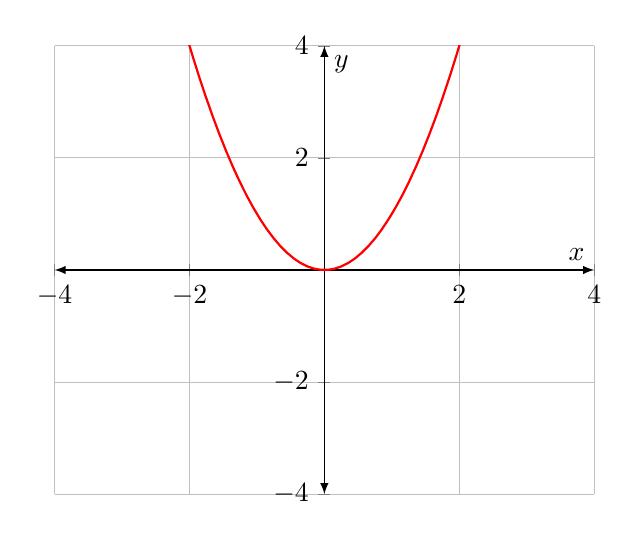
\begin{tikzpicture}
  \begin{axis}[
      grid=both,
      xmin=-4, xmax=4,
      ymin=-4, ymax=4,
      xlabel = $x$,
      ylabel = {$y$},
      axis lines=middle,
      axis line style={latex-latex}]
  \addplot+[<->,mark=none,line width=1pt][
      thick,
      domain=-10:10, 
      samples=200, 
      color=red,
  ]
  {x^2};
  \end{axis}
  \end{tikzpicture}
\end{center}

\newpage

\problem{4}{Images}
You can make some really pretty images and figures in LaTeX too!

\vspace{7em}

\begin{figure}[h]
  \centering
  
\includegraphics[width=.8\linewidth]{CMU.png}
  \caption{CMU}
  \label{fig:CMU}
\end{figure}

\vspace{7em}

\begin{figure}[h]
  \begin{subfigure}[t]{0.33\textwidth}
    \centering
    
\includegraphics[width=.8\linewidth]{amzn.png}
    \caption{Amazon}
    \label{fig:Amazon}
  \end{subfigure}
  \begin{subfigure}[t]{0.33\textwidth}
    \centering
    
\includegraphics[width=.8\linewidth]{apple.png}
    \caption{Apple}
    \label{fig:Apple}
  \end{subfigure}
  \begin{subfigure}[t]{0.33\textwidth}
    \centering
    
\includegraphics[width=.8\linewidth]{fb.png}
    \caption{Facebook}
    \label{fig:Facebook}
  \end{subfigure}
  \begin{subfigure}[t]{0.33\textwidth}
    \centering
    
\includegraphics[width=.8\linewidth]{goog.png}
    \caption{Google}
    \label{fig:Google}
  \end{subfigure}
  \begin{subfigure}[t]{0.33\textwidth}
    \centering
    
\includegraphics[width=.8\linewidth]{msft.png}
    \caption{Microsoft}
    \label{fig:Microsoft}
  \end{subfigure}
  \begin{subfigure}[t]{0.33\textwidth}
    \centering
    
\includegraphics[width=.8\linewidth]{netf.png}
    \caption{Netflix}
    \label{fig:Netflix}
  \end{subfigure}
  \caption{FAANG logos}
  \label{fig:FAANG}
\end{figure}

\vspace{7em}

and can reference back to them! Take me to \nameref{fig:FAANG} or take me to  \nameref{fig:CMU}.

\end{document}
